In structural finite element analysis, non-metal materials such as rubber and biological tissues are often encountered. Because the mechanical properties of these materials are very different from the mechanical properties of metal materials, such as large elastic deformation, incompressibility, viscoelasticity, etc. Researchers and engineers classify these materials as hyperelastic materials, and group the mechanical models that describe such materials as hyperelastic models.
\begin{figure}[H]
    \centering
    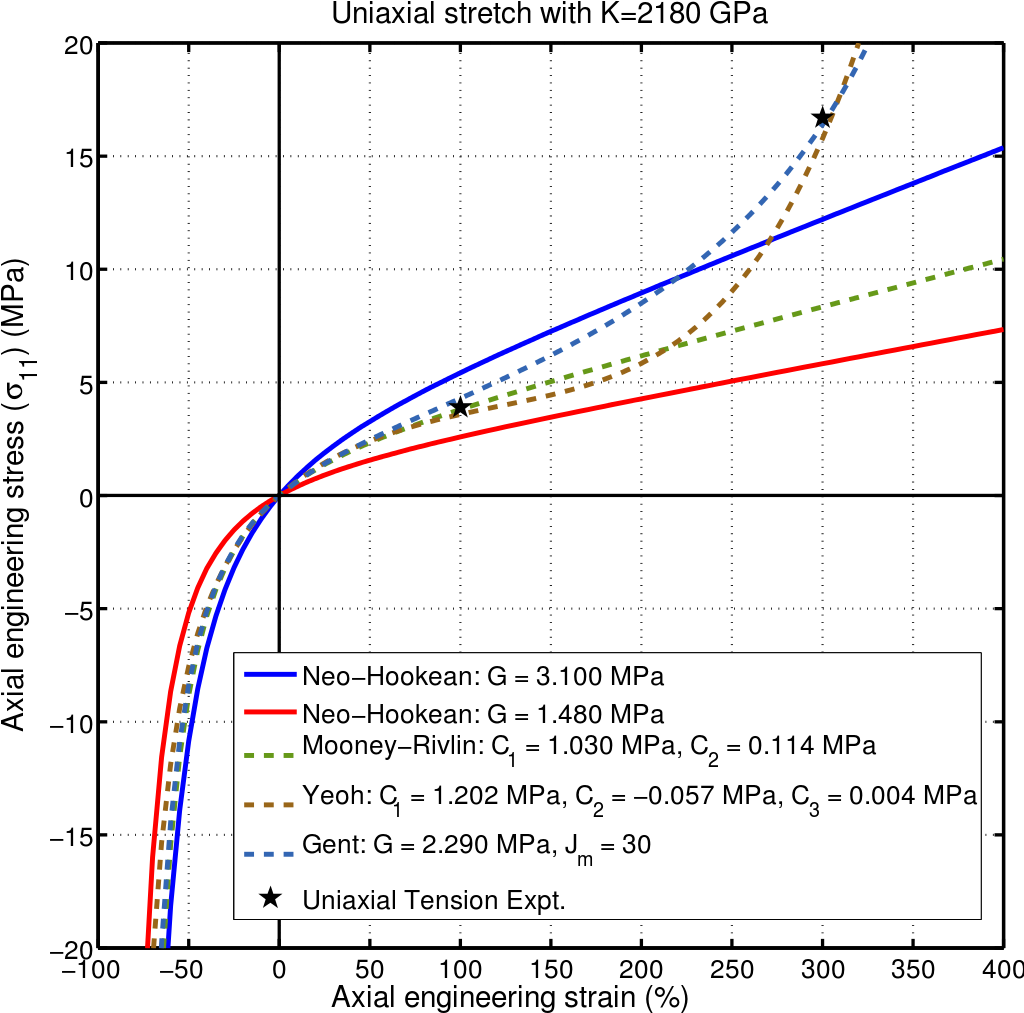
\includegraphics[scale=0.35]{Figure2/Chap3/diffhyper.png}
    \caption{The difference between elastic and hyperelastic materials in stress-strain relationship}
    \label{fig:my_label}
\end{figure}

Material behavior is described by its constitutive
relation when subjected to deformation or deformation history. Different constitutive relations can represent different material behaviors. The St. Venant–Kirchhoff
material provides a linear relation between stress and strain, which is a
simple extension of the one used for linear elastic materials. Unfortunately, this
model provides meaningful results only when the strains are small because most
materials show a nonlinear relation for large deformation. It is important to employ
a constitutive model that is appropriate for the material, the structure, and the finite
element formulation.

When the material status can completely be describable with a given total strain,
the constitutive relation is called hyperelasticity. In such a material, a strain energy density exists as a function of strain, and stress can be obtained by differentiating
the strain energy density with respect to strain. This material model is independent
of deformation history; i.e., the same deformation is expected if the final load is the
same. Rubberlike materials or human tissues belong in this category. On the other
hand, when the constitutive relation is given in terms of the stress and strain rates, it
is called hypoelasticity, which is often used in describing the plastic behavior of
materials. In such a material, the deformation history must be followed to calculate
stress because two states that have the same strain may have different stresses
depending on the loading history. Hyperelastic materials will be discussed in this
section, while hypoelastic materials will be discussed in Chap. 4. In this section, the
static response of hyperelastic materials is formulated based on the material
description, i.e., the total Lagrangian formulation. Different hyperelastic materials
will be introduced, but the main development will be explained using the Mooney-
Rivlin material, which is the most popular material model. In general, hyperelastic
materials exhibit the property of being incompressible during finite deformation;
i.e., the volume of the material is preserved. This is a common behavior of many
elastic materials in finite deformation. Numerically, a constraint, $J = 1$, needs to be
imposed to make the material incompressible. However, this causes numerical
difficulties called volumetric locking. Due to incompressibility, the hydrostatic
portion of stress cannot be calculated from the volumetric strain. The penalty
method , the selective reduced integration method , and the mixed formula-
tion method have been successfully used for incompressible and nearly
incompressible materials.

If a strain energy density exists, such that stress can be obtained from the
derivative of the strain energy with respect to strain, the system is called path
independent. Thus, it is theoretically possible to solve the nonlinear equilibrium
equation for the given total magnitude of applied load. However, this equation is
still solved by using the incremental force method with a number of load steps to
finally reach the total applied load for computational purposes. The hyperelasticity
problem contains both material nonlinearity from constitutive relations and geometric nonlinearity from kinematics.

These hyperelastic materials (models) have the following significant characteristics:
\begin{itemize}
    \item Can withstand large elastic (recoverable) deformation, sometimes with stretch up to $1000\%$.
    \item Hyperelastic materials are almost incompressible. Because the deformation is caused by the straightening of the molecular chain of the material, the volume change under the applied stress is small.
    \item The stress-strain relationship is highly nonlinear. Normally, the material softens first and then hardens under tension, but hardens sharply when compressed.
\end{itemize}
%-------------------------------------
\subsection{Strain Energy Density}
Modeling engineering materials at large deformations is still an active research
area. Without elaborating details of material modeling procedures, a method that
can describe the behavior of isotropic elastic materials which undergo finite defor-
mation is presented. In hyperelasticity, the stored strain energy density is used to
compute stress. For isotropic materials, the constitutive relation has to be indepen-
dent of the coordinate frame selected because the material has the same property for
all directions. For example, the strain component E 11 cannot be used for the
constitutive relation because its value depends on the coordinate system. Thus, it
is natural that the strain energy density is defined using invariants of strain or
alternatively that of the deformation tensor. When the undeformed state is used as
the frame of reference, the three invariants of the right Cauchy–Green deformation
tensor $C$ are given as
